%% SECTION 5.3 %%
\section{Covering Numbers}

As pointed out in the previous section, we need a suitable generalization of VC theory to find a bound on the Rademacher complexity $\mathfrak{R}_n(l \circ \mathcal{F})$ for arbitrary (i.e., possibly infinite) function classes $\mathcal{F}$. We have seen that, as in the case of binary classification, the cardinality of the set $T_l(z) = \{(l(f(x_1), y_1), \dots, l(f(x_n), y_n)^{\top} \with f \in \mathcal{F}\}$ plays a significant role in bounding the Rademacher complexity of $l \circ \mathcal{F}$. When $\mathcal{F}$ is infinite, the set $T_l(z)$ will  most likely be infinite as well. Thus, we need to find a way that lets us treat points in this set that are close to each other as if they were identical. We start with the definition of \emph{covering numbers} of a class $\mathcal{F}$.

\begin{definition}
Let $d$ be a pseudometric\footnote{The only difference between a metric and a \emph{pseudo}metric is the relaxation of the \emph{positivity} property. A metric requires every pair of distinct points $x$ and $y$ to have a positive distance $d(x, y)$ from each other. In other words, $d(x, y) = 0$ always implies $x = y$ when $d$ is a metric. For a pseudometric, this need not be true, i.e., there can be points $x \neq y$ such that $d(x, y) = 0$.} on a class of functions $\mathcal{F}$ and let $\varepsilon > 0$. An \emph{$\varepsilon$-covering} of $(\mathcal{F}, d)$ is a set of functions $V \subset \mathcal{F}$ such that every function $f \in \mathcal{F}$ is within distance of at most $\varepsilon$ to some function $g \in V$. In other words, for every $f \in \mathcal{F}$ there exists $g \in V$ such that $d(f, g) \leq \varepsilon$.

The \emph{$\varepsilon$-covering number} $\mathcal{N}(\mathcal{F}, d, \varepsilon)$ of $(\mathcal{F}, d)$ is the minimum number of functions needed to form an $\varepsilon$-covering of $(\mathcal{F}, d)$, i.e.,
\[
    \mathcal{N}(\mathcal{F}, d, \varepsilon) = \inf\set{\abs{V} \with V \text{ is an } \varepsilon \text{-net of } (\mathcal{F}, d)}.
\]

Finally, an $\varepsilon$-covering $V$ of $\mathcal{F}$ is called \emph{minimal}, if $\abs{V} = \mathcal{N}(\mathcal{F}, d, \varepsilon)$.
\end{definition}

\begin{figure}
    \centering
    \begin{tikzpicture}
        \node[above right, inner sep=0] (image) at (0,0) {
            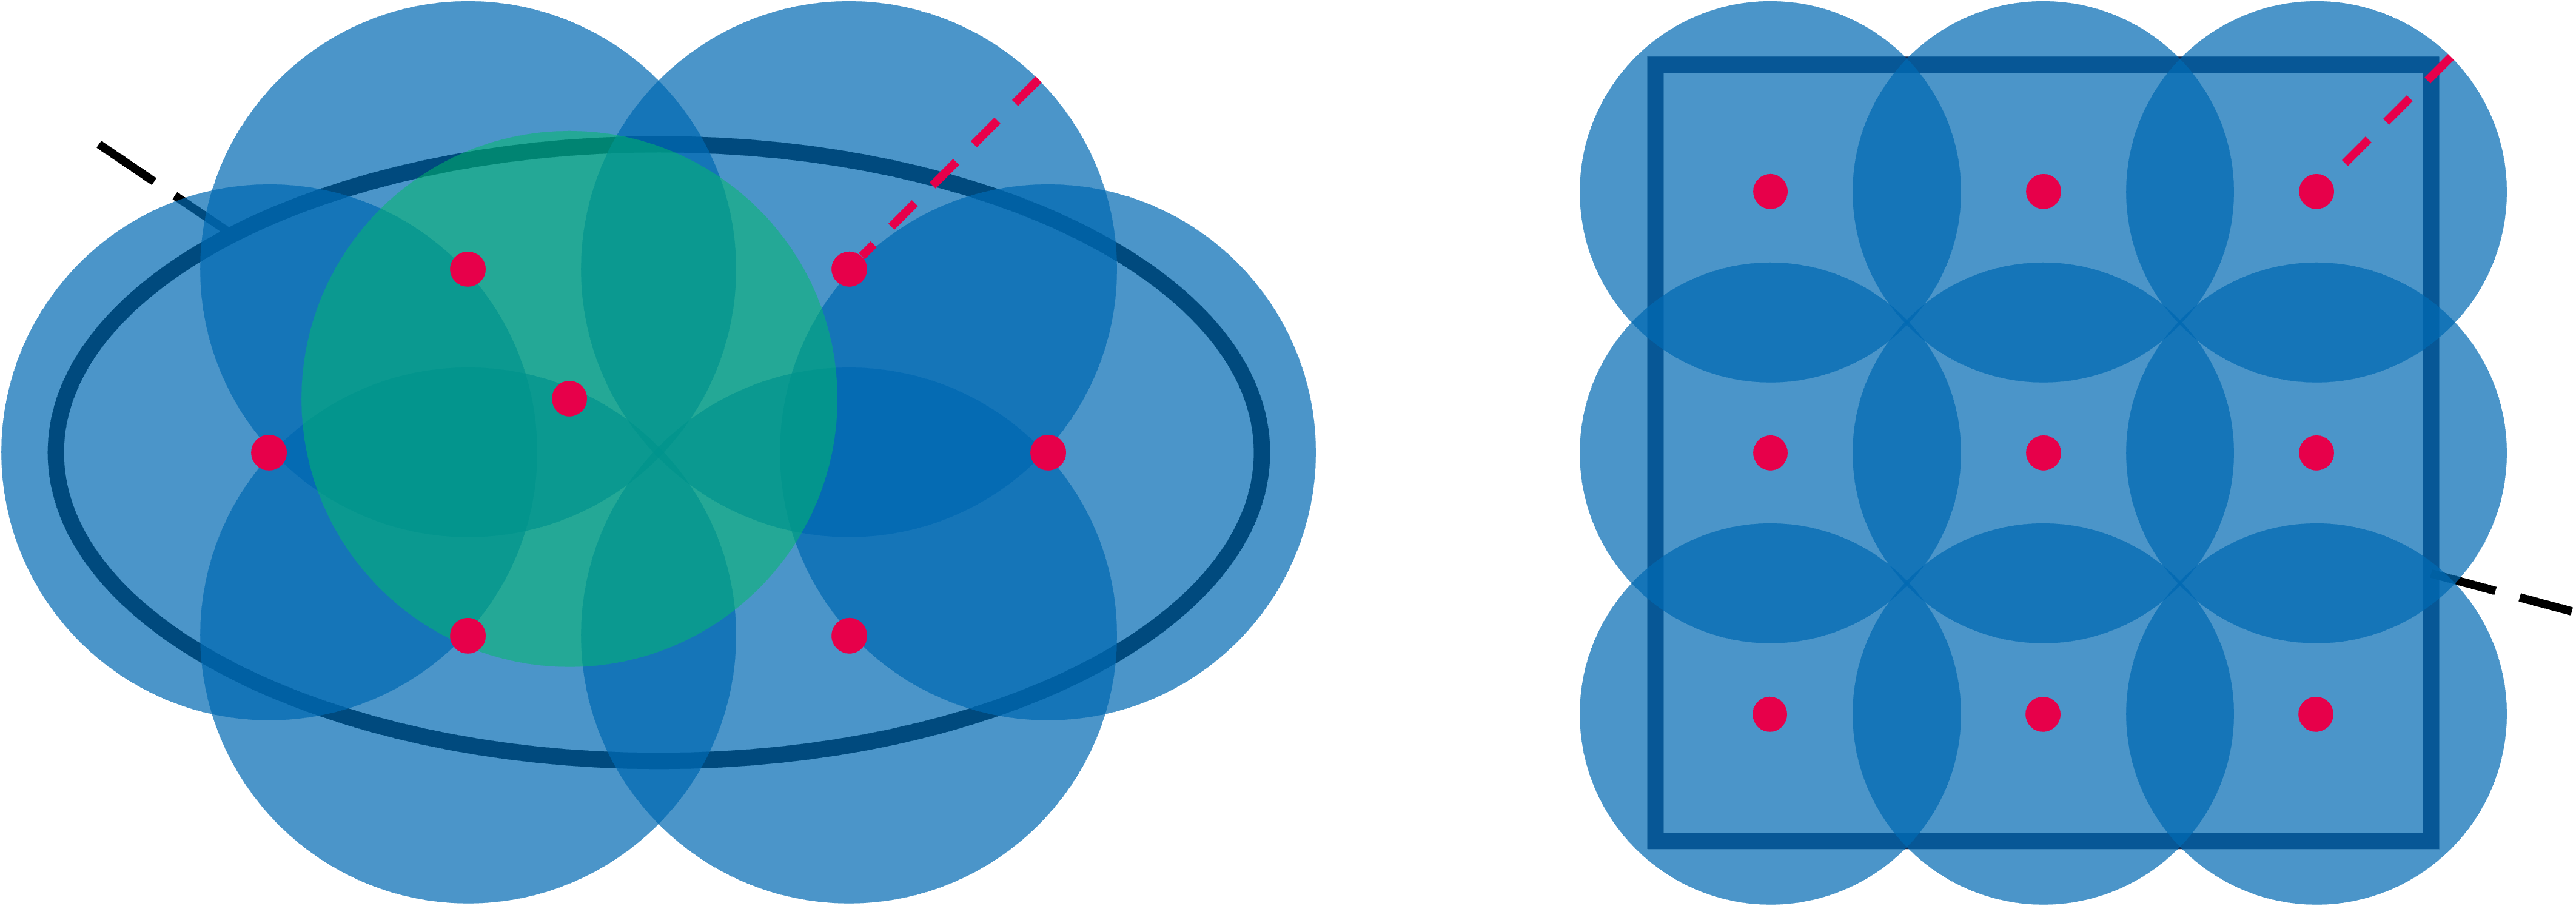
\includegraphics[width=12cm]{other/epsilon-covering}
        };

        % Create scope with normalized axes
        \begin{scope}[
            x={(image.south east)},
            y={(image.north west)}]
         
            % Grid to properly align annotations
            % \draw[help lines, step=0.1] (image.south west) grid ($(image.north east) + (0.001,0)$);

            % Annotate image
            \node[] at (0.02,0.86) {$\mathcal{F}_1$};
            \node[] at (0.36,0.90) {$\varepsilon_1$};
            \node[] at (0.09,0.46) {$g_1$};
            \node[] at (0.16,0.26) {$g_2$};
            \node[] at (0.31,0.26) {$g_3$};
            \node[] at (0.38,0.46) {$g_4$};
            \node[] at (0.31,0.66) {$g_5$};
            \node[] at (0.16,0.66) {$g_6$};
            \node[] at (0.20,0.52) {$g_7$};

            \node[] at (1.02,0.30) {$\mathcal{F}_2$};
            \node[] at (0.89,0.88) {$\varepsilon_2$};
            \node[] at (0.67,0.74) {$g_1$};
            \node[] at (0.77,0.74) {$g_2$};
            \node[] at (0.88,0.74) {$g_3$};
            \node[] at (0.67,0.46) {$g_4$};
            \node[] at (0.77,0.46) {$g_5$};
            \node[] at (0.88,0.46) {$g_6$};
            \node[] at (0.67,0.16) {$g_7$};
            \node[] at (0.77,0.16) {$g_8$};
            \node[] at (0.88,0.16) {$g_9$};
            
        \end{scope}
    \end{tikzpicture}
    \caption{%
         Coverings of two classes $\mathcal{F}_1$ and $\mathcal{F}_2$. \textbf{Left}, a class $\mathcal{F}_1$ covered by an $\varepsilon_1$-covering ${\color{red} V} = \set{{\color{red} g_1}, \dots, {\color{red} g_7}}$. Note, however, that $\mathcal{N}(\mathcal{F}, d, \varepsilon_1) < 7$ since the $\varepsilon_1$-ball centered at $g_7$ and depicted in green is redundant (i.e., the remaining 6 $\varepsilon_1$-balls still cover all of $\mathcal{F}_1$). \textbf{Right}, a class $\mathcal{F}_2$ covered by a \emph{minimal} $\varepsilon_2$-covering ${\color{red} V} = \set{{\color{red} g_1}, \dots, {\color{red} g_9}}$.
    }
    \label{fig: epsilon-covering}
\end{figure}

If $V$ is an $\varepsilon$-covering of $(\mathcal{F}, d)$, then clearly
\[
    \mathcal{F} = \bigcup_{g \in V} B_{d, \varepsilon}(g),
\]
where $B_{d, \varepsilon}(g) = \set{f \in \mathcal{F} \with d(f, g) \leq \varepsilon}$ is the closed ball of radius $\varepsilon$ centered at $g$. Thus, $\mathcal{F}$ is covered by closed balls of radius $\varepsilon$ centered on elements in $V$, hence the name $\varepsilon$-covering.

Note that the definition of $\varepsilon$-coverings is in no way restricted to classes of \emph{functions}. Instead, all of these constructions make sense on any set $M$ endowed with a pseudometric $d$.

Next, we introduce the \emph{conditional Rademacher average} of a class\footnote{In what follows, we use a general class of functions $\mathcal{F}$ and a set of points $\set{z_1, \dots, z_n}$. In the setting of empirical risk minimization, we would substitute $\mathcal{F}$ for $l \circ \mathcal{F}$ and the set under consideration would be the observations $\set{(x_1, y_1), \dots, (x_n, y_n)}$.} of functions $\mathcal{F}$ given a set of points $\set{z_1, \dots, z_n}$.

\begin{definition}
The \emph{conditional Rademacher average} of a class $\mathcal{F}$ of functions $f \colon \mathcal{Z} \to \R$ given a set of $n$ points $z = \set{z_1, \dots, z_n} \subset \mathcal{Z}$ is defined as
\[
    \hat{\mathfrak{R}}_n^z(\mathcal{F}) = \Exp\left[\sup_{f \in \mathcal{F}} \abs{\frac{1}{n} \sum_{i=1}^n \sigma_i f(z_i)}\right],
\]
where $\sigma_1, \dots, \sigma_n$ are i.i.d.\ $\Rad(\nicefrac{1}{2})$ random variables.
\end{definition}

Notice that, if $\mathcal{F}$ is a class of functions $f \colon \mathcal{Z} \to \R$, and we define the Rademacher complexity of $\mathcal{F}$ as\footnote{This is simply the generalization of Definition \ref{def: rademacher complexity for general loss} to an arbitrary class of functions $\mathcal{F}$.}
\[
    \mathfrak{R}_n(\mathcal{F}) = \sup_{z \in \power(\mathcal{Z})} \Exp\left[\sup_{f \in \mathcal{F}} \abs{\frac{1}{n} \sum_{i=1}^n \sigma_i f(z_i)}\right],
\]
where the supremum ranges over all subsets $z = \set{z_1, \dots, z_n} \in \power(\mathcal{Z})$, then clearly
\begin{equation}
\label{eq: rademacher complexity and conditional rademacher average}
    \highlightMath{
        \mathfrak{R}_n(\mathcal{F}) = \sup_{z \in \power(\mathcal{Z})} \hat{\mathfrak{R}}_n^z(\mathcal{F}).
    }
\end{equation}

There is one more term we have to introduce before we state the first result of this section.

\begin{definition}
Given a set of points $z = \set{z_1, \dots, z_n} \subset \mathcal{Z}$ and a class $\mathcal{F}$ of functions $f \colon \mathcal{Z} \to \R$, the \emph{empirical $L^1$-distance} between $f, g \in \mathcal{F}$ is given by
\[
    d_1^z(f, g) = \frac{1}{n} \sum_{i=1}^n \abs{f(z_i) - g(z_i)}.
\]
\end{definition}

With these definitions in place, we will prove an upper bound of the conditional Rademacher average of a class $\mathcal{F}$ that (besides the number of observations $n$) depends only on the $\varepsilon$-covering numbers of $\mathcal{F}$ with respect to the empirical $L^1$-distance $d_1^z$. In order for these (covering numbers) to be well-defined, we would have to show that the empirical $L^1$-distance defines a pseudometric on a given class $\mathcal{F}$ (since this is assumed to be the case in the definition of covering numbers presented earlier). This is indeed true, and it follows directly from the properties of the absolute value.

\begin{theorem}
\label{thm: bound on conditional rademacher average}
Let $\mathcal{F}$ be a class of functions $f \colon \mathcal{Z} \to [-1, 1]$, and let $z = \set{z_1, \dots, z_n} \subset \mathcal{Z}$ be a set of $n$ points. Then,
\[
    \hat{\mathfrak{R}}_n^z(\mathcal{F}) \leq \inf_{\varepsilon > 0} \varepsilon + \sqrt{\frac{2 \log(2 \mathcal{N}(\mathcal{F}, d_1^z, \varepsilon))}{n}}.
\]
\end{theorem}

\begin{proof}
We can assume $\mathcal{N}(\mathcal{F}, d_1^z, \varepsilon) < \infty$, since the inequality is trivially true otherwise. Given $\varepsilon > 0$, we let $V_{\varepsilon}$ be a minimal $\varepsilon$-covering of $\mathcal{F}$, i.e., $\abs{V_{\varepsilon}} = \mathcal{N}(\mathcal{F}, d_1^z, \varepsilon) < \infty$. For every function $f \in \mathcal{F}$, there exists $f^{\circ} \in V_{\varepsilon}$ such that $d_1^z(f, f^{\circ}) \leq \varepsilon$. By the triangle inequality, we have
\[
    \hat{\mathfrak{R}}_n^z(\mathcal{F}) = \Exp\left[\sup_{f \in \mathcal{F}} \frac{1}{n} \abs{\sum_{i=1}^n \sigma_i f(z_i)}\right] \leq \Exp\left[\sup_{f \in \mathcal{F}} \frac{1}{n} \abs{\sum_{i=1}^n \sigma_i (f(z_i) - f^{\circ}(z_i))}\right] + \Exp\left[\sup_{f \in \mathcal{F}} \frac{1}{n} \abs{\sum_{i=1}^n \sigma_i f^{\circ}(z_i)}\right].
\]
The triangle inequality also implies
\[
    \frac{1}{n} \abs{\sum_{i=1}^n \sigma_i (f(z_i) - f^{\circ}(z_i))} \leq \frac{1}{n} \sum_{i=1}^n \abs{f(z_i) - f^{\circ}(z_i)} = d_1^z(f, f^{\circ}) \leq \varepsilon,
\]
since $\abs{\sigma_i} = 1$ almost surely. Hence,
\[
    \hat{\mathfrak{R}}_n^z(\mathcal{F}) \leq \varepsilon + \Exp\left[\sup_{f \in \mathcal{F}} \frac{1}{n} \abs{\sum_{i=1}^n \sigma_i f^{\circ}(z_i)}\right].
\]
As $f^{\circ} \in V_{\varepsilon}$, we obtain
\[
    \Exp\left[\sup_{f \in \mathcal{F}} \frac{1}{n} \abs{\sum_{i=1}^n \sigma_i f^{\circ}(z_i)}\right] = \Exp\left[\max_{g \in V_{\varepsilon}} \frac{1}{n} \abs{\sum_{i=1}^n \sigma_i g(z_i)}\right] = \mathfrak{R}_n(B),
\]
where $\mathfrak{R}_n(B)$ denotes the Rademacher complexity of the \emph{finite} set $B = \set{(g(z_1), \dots, g(z_n))^{\top} \with g \in V_{\varepsilon}} \subset \R^n$. Since every $g \in V_{\varepsilon} \subset \mathcal{F}$ takes values in $[-1, 1]$, we have $\max_{b \in B} \norm{b}_2 \leq \sqrt{n}$, and Lemma \ref{lem: bound on rademacher complexity of finite set} hence tells us that
\[
    \mathfrak{R}_n(B) \leq \sqrt{\frac{2 \log(2 \abs{B})}{n}} \leq \sqrt{\frac{2 \operatorname{log}(2 \abs{V_{\varepsilon}})}{n}} = \sqrt{\frac{2 \operatorname{log}(2 \mathcal{N}(\mathcal{F}, d_1^z, \varepsilon))}{n}},
\]
since $\abs{B} \leq \abs{V_{\varepsilon}} = \mathcal{N}(\mathcal{F}, d_1^z, \varepsilon)$. Altogether,
\[
    \hat{\mathfrak{R}}_n^z(\mathcal{F}) \leq \varepsilon + \Exp\left[\sup_{f \in \mathcal{F}} \frac{1}{n} \abs{\sum_{i=1}^n \sigma_i f^{\circ}(z_i)}\right] \leq \varepsilon + \sqrt{\frac{2 \operatorname{log}(2 \mathcal{N}(\mathcal{F}, d_1^z, \varepsilon))}{n}}.
\]
Since this is true for every $\varepsilon > 0$, we can take the infimum over $\varepsilon$ to arrive at the desired result.
\end{proof}

Observe that there is a trade-off in the upper bound of the previous result, since the $\varepsilon$-covering numbers $\mathcal{N}(\mathcal{F}, d_1^z, \varepsilon)$ of $\mathcal{F}$ increase as $\varepsilon$ decreases, and vice versa. Next, we introduce another set of empirical distances.

\begin{definition}
Given a set of points $z = \set{z_1, \dots, z_n} \subset \mathcal{Z}$ and a class $\mathcal{F}$ of functions $f \colon \mathcal{Z} \to \R$, the \emph{empirical $L^p$-distance} between $f, g \in \mathcal{F}$ is given by
\[
    d_p^z(f, g) = \left(\frac{1}{n} \sum_{i=1}^n \abs{f(z_i) - g(z_i)}^p \right)^{\nicefrac{1}{p}}, \quad p \geq 1.
\]
For $p = \infty$, we set
\[
    d_{\infty}^z(f, g) = \max_{1 \leq i \leq n} \abs{f(z_i) - g(z_i)}.
\]
\end{definition}

Before we proceed to state the next result on $\varepsilon$-covering numbers, we recall a special case of H{\"o}lder's inequality.

\begin{proposition}[H{\"o}lder, 1889]
\label{prop: hoelder}
For any $r, s \geq 0$, and $x, y \in \R^n$, it holds
\[
    \left(\sum_{i=1}^n \abs{x_i}^r \abs{y_i}^s \right)^{r+s} \leq \left(\sum_{i=1}^n \abs{x_i}^{r+s}\right)^r \left(\sum_{i=1}^n \abs{y_i}^{r+s}\right)^s.
\]
\end{proposition}

It is clear that the $\varepsilon$-covering numbers of a class $\mathcal{F}$ decrease as $\varepsilon$ increases. Essentially, this is due to the fact that the open balls $B_{d, \varepsilon}(f)$ increase in size\footnote{More precisely, $\varepsilon > \varphi$ implies $B_{d, \varepsilon}(f) \supset B_{d, \varphi}(f)$.} for larger $\varepsilon$, i.e.,
\[
    \varepsilon \uparrow \quad \Rightarrow \quad \text{size of } B_{d, \varepsilon}(f) \uparrow \quad \Rightarrow \quad \mathcal{N}(\mathcal{F}, d, \varepsilon) \downarrow.
\]
We will now show that something similar in spirit is true for the family of empirical distances $d_p^z$ we have defined above, namely,
\[
    p \uparrow \quad \Rightarrow \quad \text{size of } B_{d_p^z, \varepsilon}(f) \downarrow \quad \Rightarrow \quad \mathcal{N}(\mathcal{F}, d_p^z, \varepsilon) \uparrow.
\]

\begin{proposition}
Let $\mathcal{F}$ be a class of functions $f \colon \mathcal{Z} \to \R$ and fix a set of points $z = \set{z_1, \dots, z_n}$. For $1 \leq p \leq q < \infty$ and $\varepsilon > 0$, it holds
\[
    \mathcal{N}(\mathcal{F}, d_p^z, \varepsilon) \leq \mathcal{N}(\mathcal{F}, d_q^z, \varepsilon) \leq \mathcal{N}(\mathcal{F}, d_{\infty}^z, \varepsilon).
\]
\end{proposition}

\begin{proof}
Throughout this proof, let us write $u_i = f(z_i) - g(z_i)$ and $u = \max_{1 \leq i \leq n} \abs{u_i}$. We first tackle the inequality $\mathcal{N}(\mathcal{F}, d_q^z, \varepsilon) \leq \mathcal{N}(\mathcal{F}, d_{\infty}^z, \varepsilon)$. Since the functions $x \mapsto x^q$ and $x \mapsto x^{\nicefrac{1}{q}}$ are increasing on $[0, \infty)$, we have
\[
    d_q^z(f, g) = \left(\frac{1}{n} \sum_{i=1}^n \abs{u_i}^q\right)^{\nicefrac{1}{q}} \leq \left(\frac{1}{n} \sum_{i=1}^n u^q\right)^{\nicefrac{1}{q}} = u = \max_{1 \leq i \leq n} \abs{u_i} = d_{\infty}^z(f, g).
\]
If $g \in B_{d_{\infty}^z, \varepsilon}(f)$, so that $d_{\infty}^z(f, g) < \varepsilon$, then the above inequality implies $d_q^z(f, g) \leq d_{\infty}^z(f, g) < \varepsilon$. Hence, $B_{d_{\infty}^z, \varepsilon}(f) \subset B_{d_q^z, \varepsilon}(f)$. This, in turn, implies that every $\varepsilon$-covering of $\mathcal{F}$ w.r.t.\ $d_{\infty}^z$ defines an $\varepsilon$-covering of $\mathcal{F}$ w.r.t.\ $d_q^z$, and thus, $\mathcal{N}(\mathcal{F}, d_q^z, \varepsilon) \leq \mathcal{N}(\mathcal{F}, d_{\infty}^z, \varepsilon)$.

To prove the inequality $\mathcal{N}(\mathcal{F}, d_p^z, \varepsilon) \leq \mathcal{N}(\mathcal{F}, d_q^z, \varepsilon)$, we will make use of the version of H{\"o}lder's inequality stated in Proposition \ref{prop: hoelder}. With $r = \frac{1}{p} - \frac{1}{q} \geq 0$ and $s = \frac{1}{q} \geq 0$, we have $r + s = \frac{1}{p}$, and hence
\begin{align*}
    d_p^z(f, g) = \left(\frac{1}{n} \sum_{i=1}^n \abs{u_i}^p\right)^{\nicefrac{1}{p}} &= n^{-\nicefrac{1}{p}} \left(\sum_{i=1}^n \abs{1}^r \abs{u_i^{pq}}^s\right)^{r+s} \\[4pt]
    &\leq n^{-\nicefrac{1}{p}} \left(\sum_{i=1}^n \abs{1}^{r+s}\right)^r \left(\sum_{i=1}^n \abs{u_i^{pq}}^{r+s}\right)^s = n^{-\nicefrac{1}{q}} \left(\sum_{i=1}^n \abs{u_i}^{q}\right)^{\nicefrac{1}{q}} = d_q^z(f, g).
\end{align*}
By the same logic as before, the inequality $d_p^z(f, g) \leq d_q^z(f, g)$ implies $\mathcal{N}(\mathcal{F}, d_p^z, \varepsilon) \leq \mathcal{N}(\mathcal{F}, d_q^z, \varepsilon)$.
\end{proof}
